%%%%%%%%%%%%%%%%%%%%%%%%%%%%%%%%%%%%%%%%%%%%%%%%%%%%%%%%%%%%%%%%%%
\section{Introduction}\label{intro}

%% Goals of the intro
% Why are we studying this problem
% Context of our work (previous work)
% Motivation for this work (our idea)
% Summary of our contribution
% Summary of our results



% Heavy change in the motivation, the second half of the original
% paragraph was quite hard to understand.
Earthquakes can cause great damage to human society through soil
rupture, movement, tsunami, etc. Some recent earthquakes that
highlight this destructive potential are the great East Japan
Earthquake of 2011 (depicted in figure\ref{GreatEastJapan}), and the
April 2015 earthquake in Nepal. One important tool for the enactment
of policies that minimize the consequences of these events are
earthquake occurrence models (also called risk models). These models
can be used to identify patterns in the seismic mechanisms that
generate earthquakes, and are important to increase our understanding
of these events.


%% It would be VERY GOOD if we could replace this figure with a new 
%% One of the same area/location with the earthquakes colored by 
%% cluster. This would reinforce the clustering characteristic of the 
%% paper.
%\begin{figure}[]
%\centering
%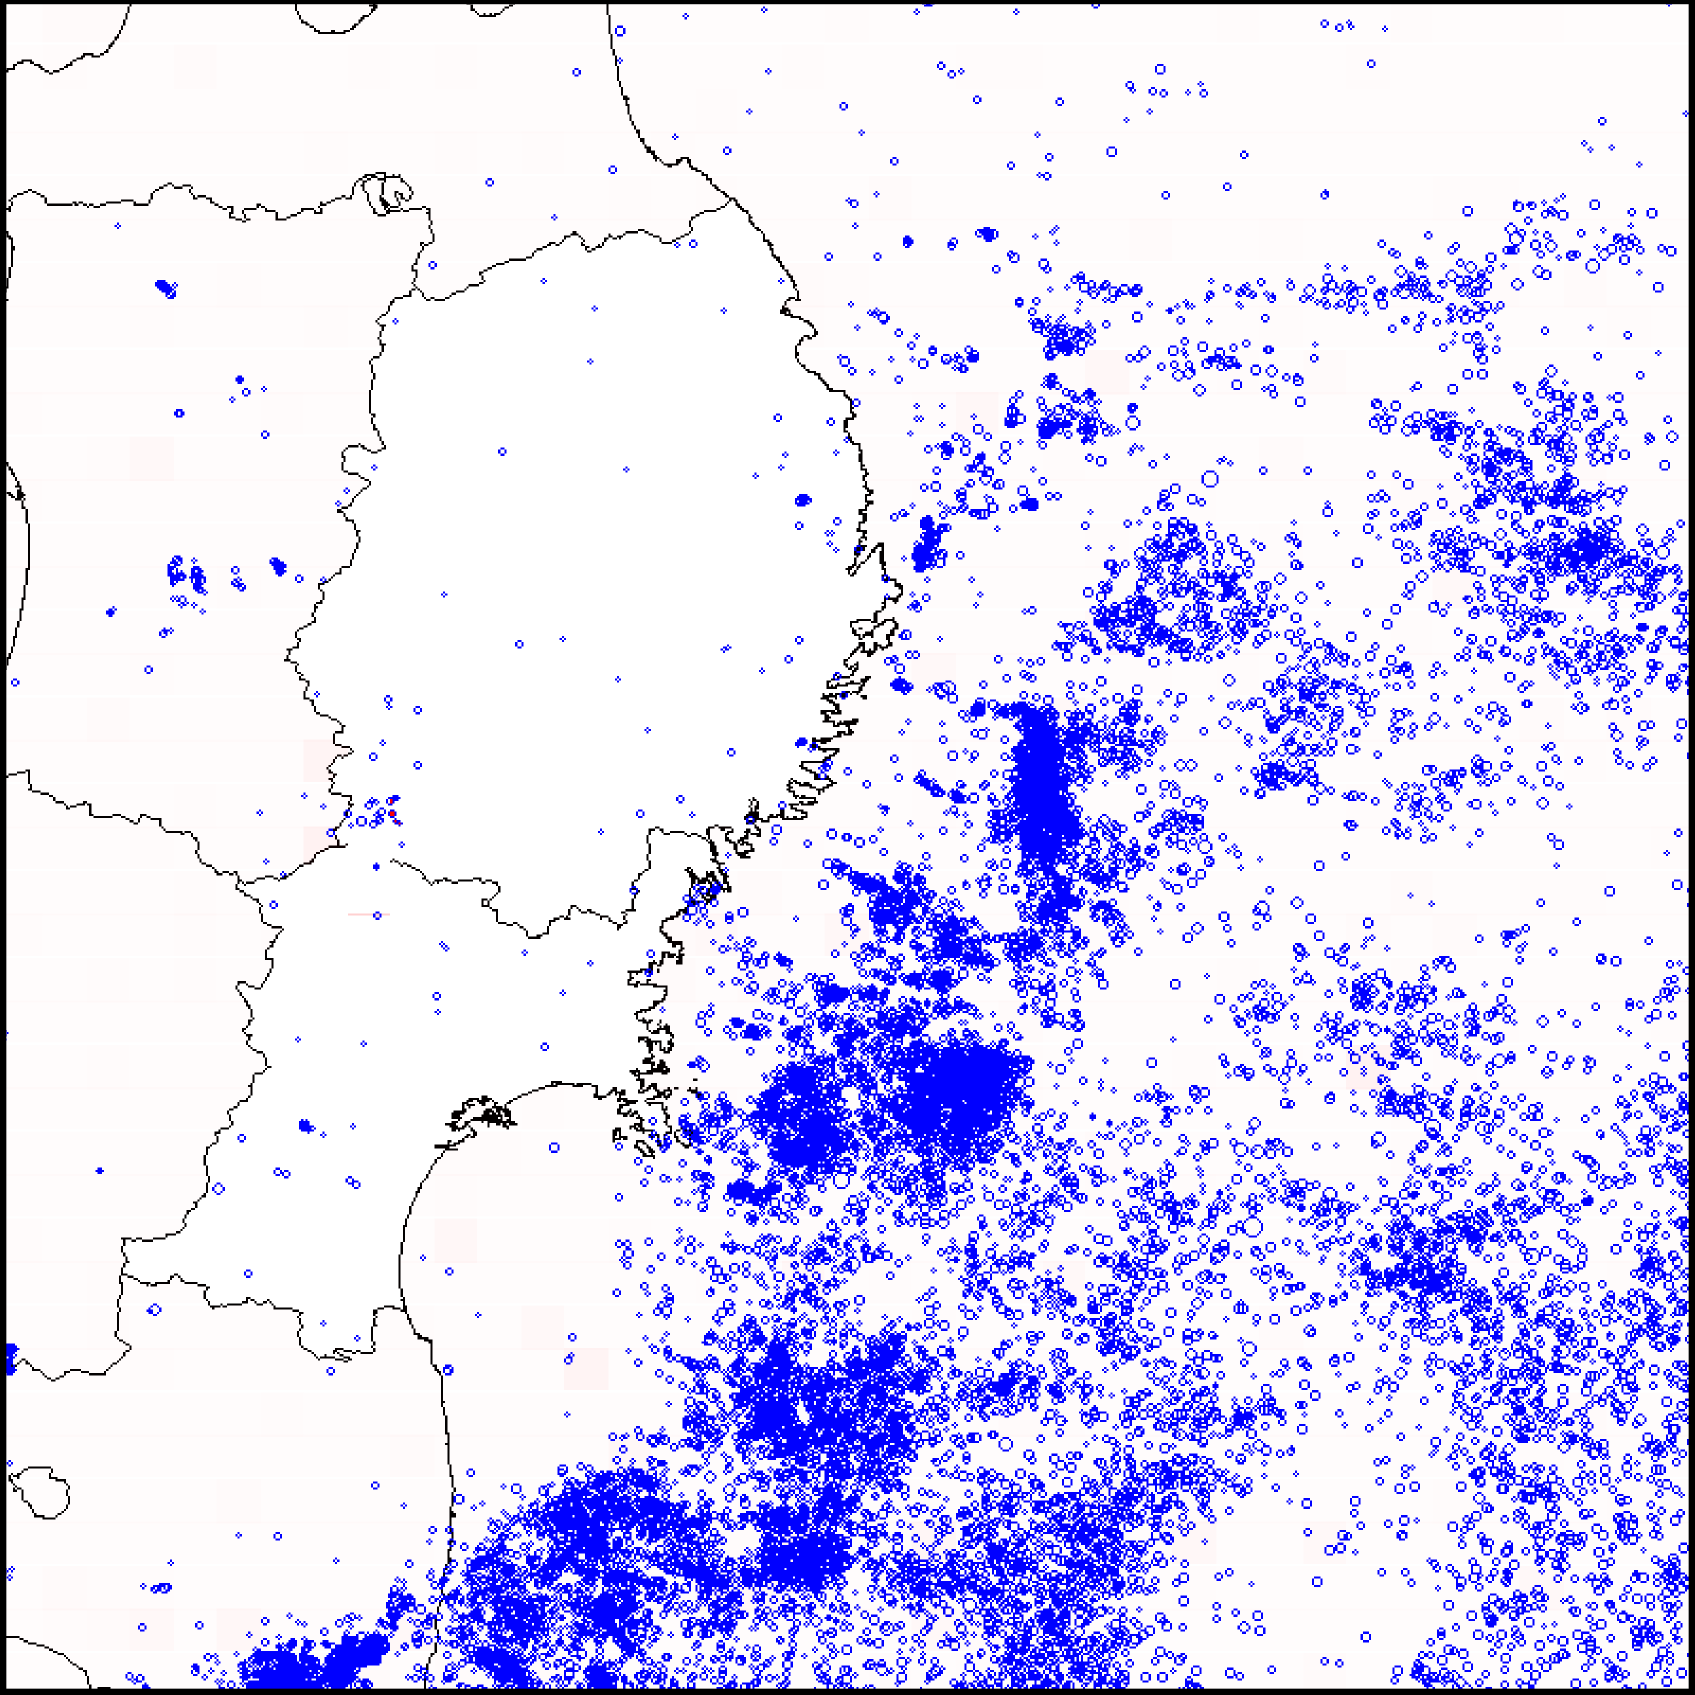
\includegraphics[width=.45\textwidth]{img/earthquakes2011.png}
%\caption{Seismic Activity in Eastern Japan in 2011. Each blue dot
%  represents one earthquake}
%\label{GreatEastJapan}
%\end{figure}

%this figure I got from Gabriels work. It shows earthquake clusters from 2003 to 2011. It doesnt look too good for me. Maybe we can take a look at Gabriels code and adapt it
\begin{figure}[]
	\centering
	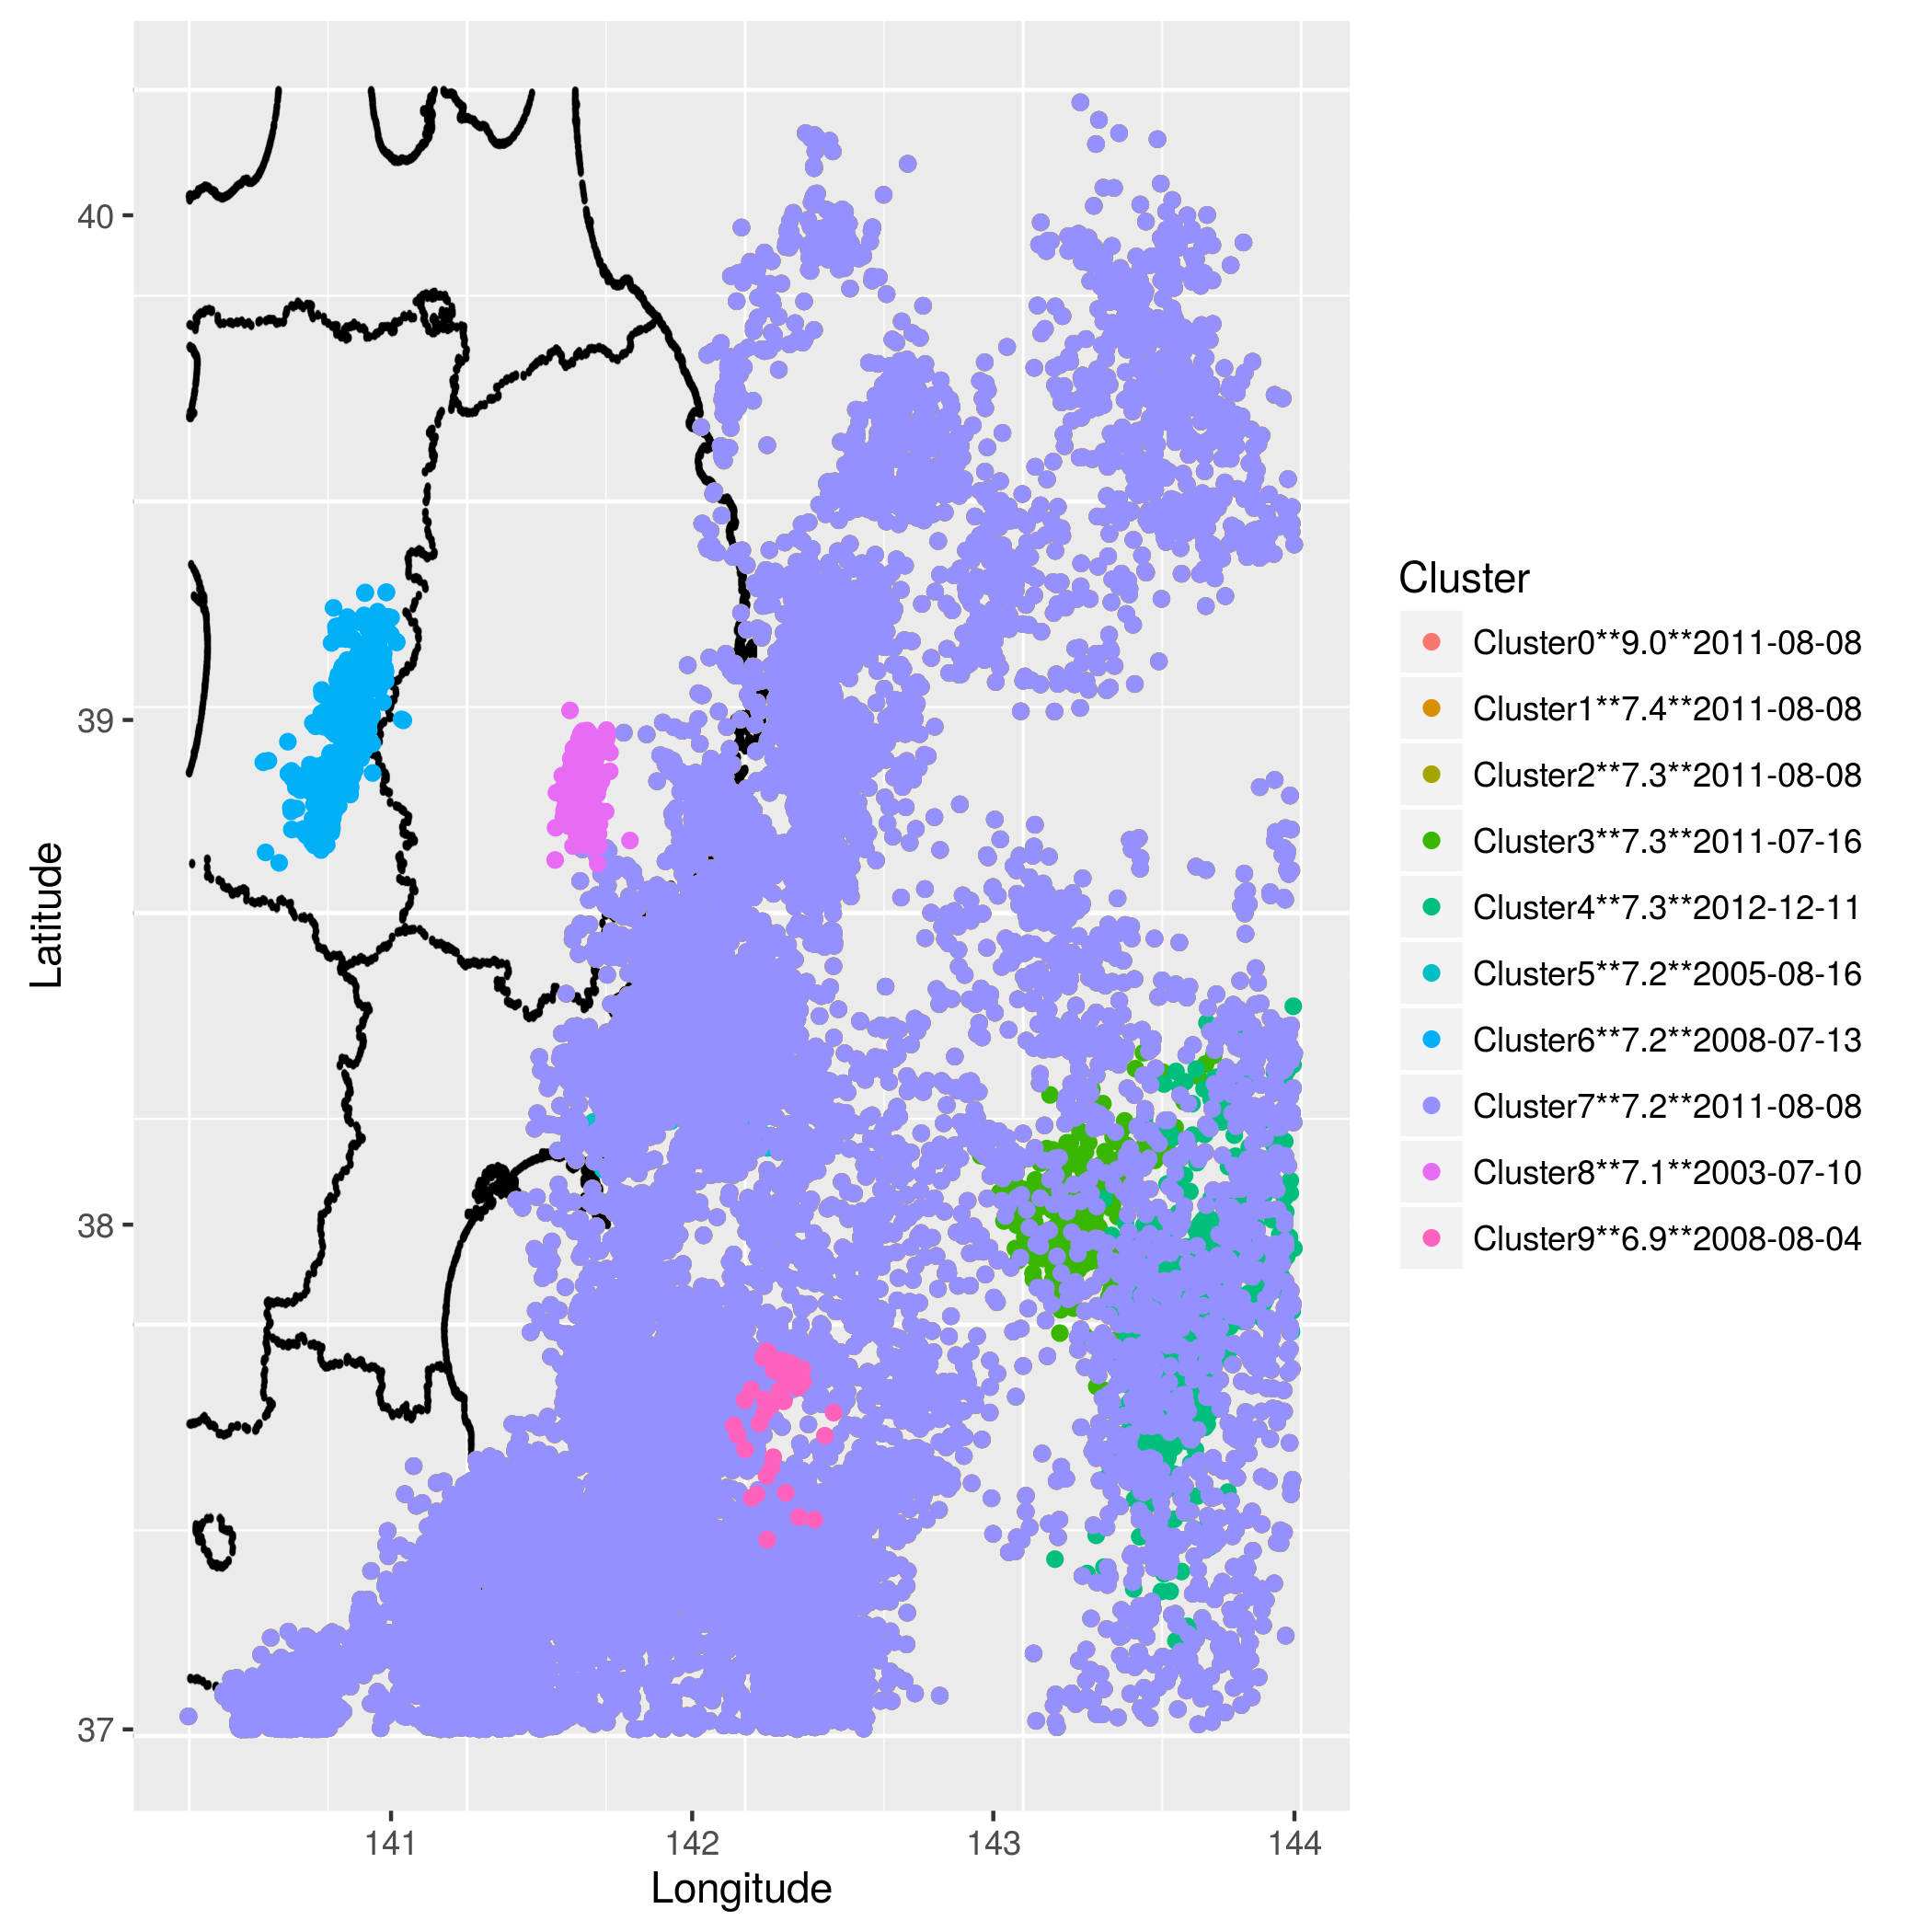
\includegraphics[width=.55\textwidth]{img/slc_leste.png}
	\caption{Seismic Activity in Eastern Japan during the years of 2003 to 2011.}
	\label{GreatEastJapan}
\end{figure}

In our previous work~\cite{ecta14}, we proposed a way to generate
earthquake risk models using a standard Genetic Algorithm (here called
the GAModel). The GA model was shown to be competitive with the
Relative Intensity (RI) model, while not using any a-priori
information about the distribution of earthquake occurrences. However,
we have identified a number of issues with the GAModel. Addressing
these issues will be the focus of this paper.

The first issue was that the GAModel used a genome representation for
the risk model with a too large number of parameters (over 2000 for
regular cases). In the final models evolved, the parameters with least
importance for a certain scenario would show random drift in their
values, indicating that they were not contributing for the overall
model.  To address this issue, we proposed the ReducedGAModel. The
basic idea of the ReducedGAModel is that only areas with a minimal
probability of earthquake occurrence are represented as parameters in
evolutionary process. We expect that changing the representation in
this way may increase the convergence speed of the evolutionary
process.

The second issue was that GAModel did not take into account any 
sort of domain knowledge, such as the assumption that earthquakes
cluster in both time and space.
% End of current changes
%%%%%%%%%%%%%%%%%%%%%%%%%%%%%%%%%%%%%%%%%%%%%%%%%%%%%%%%%%%%%%%%%%%

%% TODO:
% Second issue, we do not use domain knowledge. Risk is assigned randomly
% Solution, emp-GAmodel, where we generate only ``main shocks'' first,
% and generate aftershocks from the main shocks using ETAS.

% In this paper we will explore EMPGA and ReducedGA separately, as well as 
% In concert (ADD new 2x2 figure/table here)

% Third issue, clustering. ``it is known'' that clustering earthquakes
% and removing aftershocks may make earthquake catalogs easier to analyse
% In this sense, we use two different clustering techniques, and 
% Test the above GAmodel variations in the clustered catalog as well

% The results show which approaches improve on the results of the 
% Original GAModel, and which do not offer any significant contribution

% Suggestion: new section division:
% Section 1- Introduction
% Section 2- Bibliography and GAmodel review
% Section 3- Reduced GA and EMP-GA
% Section 4- Clustering the catalog
% Section 5- Experiments
% Section 6- Discussion of the results
% Section 7- Conclusions


%%%%%%%%%%%%%%%%%%%%%%% Untouched text %%%%%%%%%%%%%%%%%%%%%%%%%
The other idea is based on the assumption that earthquakes cluster in
both space and time, and we want incorporate in the Genetic Algorithm
technique (GA) some geophysical knowledge. It is a hybridisation of
the models generated with GA some empirical laws, such as the modified
Omori law. First, the background intensity (the independent
earthquakes or mainshocks), which is a function of the space, is
forecast using the GA. Then, we use some empirical laws to obtain the
dependent earthquakes (aftershocks) for a specific time interval.

The Emp-GAModel is a method proposed that incorporates some
geophysical knowledge. It is a hybridization of the models generated
by the GAModel with the these empirical laws, see Section
\ref{Models}.

Finally, there is the Emp-ReducedGAModel. This method is a combination
of the two ideas. Therefore, it also performs a hybridization of
models with the group of empirical law. Though, for this method, the
models are generated by the ReducedGAModel.

The forecast models produced by those methods and the ones produced by
the GAModel were all analyzed by their log-likelihood values
calculated as suggested by the Regional Earthquake Likelihood Model
(RELM)~\cite{schorlemmer2007earthquake}.

For developing the methods and to be able to compare them we used the
earthquake catalog from the Japanese Meteorological Agency (JMA),
using event data from 2005 to 2010.

This paper is organized as: in Section \ref{estadoArte}reviews
applications of Evolutionary Computation in the context of seismology
research. The next Section,Section \ref{Models}, we give a details of
each of the forecast proposed covering the Collaboratory for the Study
of Earthquake Predictability (CSEP) framework and the empirical
laws. In Section \ref{Tests}, we give the description of the tests
proposed in~\cite{Schorlemmer2007}. After that, in \ref{exp}, we
define the target areas used for the experiment and the data from the
JMA; we clarify the design followed during the experiments and how we
compared the forecast models derived from our methods. Finally, we
show the results and conclude this work in~\ref{Results} and
\ref{Conclusions}.
